\begin{frame}
	\frametitle{Em Geral...}
	\begin{center}
		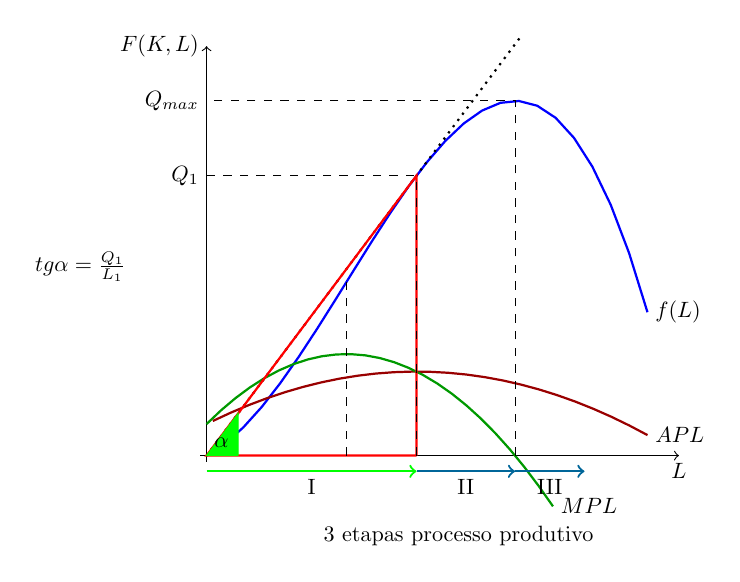
\begin{tikzpicture}[
			scale = 0.8,
			every node/.style = {scale = 0.8},
			declare function = {
				f(\x)=1*(\x/2)+2*(\x/2)^2-0.6*(\x/2)^3;
				apl(\x) = f(\x)/\x;
				mpl(\x) = 1/2+\x-0.225*\x^2;
				tgt(\x) = 0 + apl(10/3)*\x;
			}
			]

			\draw[->] (-0.1,0) -- (7.5,0) node[below]{$L$};
			\draw[->] (0,-0.1) -- (0,6.5) node[left]{$F(K,L)$};

			\draw[blue,thick,domain = 0:7,variable=\x,samples=25] plot (\x,{f(\x)});
			\draw[red!60!black,thick,domain = 0.1:7,variable=\x,samples=25] plot (\x,{apl(\x)});
			\draw[green!60!black,thick,domain = 0:5.5,variable=\x,samples=25] plot (\x,{mpl(\x)});

			\onslide<2->{
				\draw[dotted,thick,domain=0:5,variable=\x] plot (\x,{tgt(\x)});
			}

			\onslide<3-5>{
				\draw[red,thick] ({10/3},0) -- ({10/3},{f(10/3)}) -- (0,0) -- ({10/3},0);
			}

			\onslide<4-5>{
				\draw[green,fill] ({1.5/3},0) -- ({1.5/3},{tgt(1.5/3)}) -- (0,0) -- ({1.5/3},0);
				\draw(0,0) node[above right]{$\alpha$};
			}

			\only<5>{
				\draw(-2,3) node[]{\(tg\alpha=\frac{Q_1}{L_1}\)};
			}

			\onslide<1-5>{
				\draw(7,{f(7)}) node[right]{$f(L)$};
				\draw(7,{apl(7)}) node[right]{$APL$};
				\draw(5.5,{mpl(5.5)}) node[right]{$MPL$};
			}

			\draw[dashed] ({20/9},0) --({20/9},{f(20/9)});
			\draw[dashed] (4.89813,0) -- (4.89813,{f(4.89813)}) -- (0,{f(4.89813)})node[left]{$Q_{max}$};
			\draw[dashed] ({10/3},0) -- ({10/3},{f(10/3)}) -- (0,{f(10/3)})node[left]{$Q_1$};

			\onslide<6->{
				\draw[->,thick,green] (0,-0.25) -- ({10/3},-0.25) node[black,midway,yshift=-0.25cm]{I};
				\draw[->,thick,blue!60!green] ({10/3},-0.25) -- (4.89813,-0.25)node[black,midway,yshift=-0.25cm]{II};
				\draw[->,thick,blue!60!green] (4.89813,-0.25) -- (6,-0.25)node[black,midway,yshift=-0.25cm]{III};

				\draw(4,-1) node[below]{3 etapas processo produtivo};
			}
		\end{tikzpicture}
	\end{center}

	\onslide<6->{Etapa II: Zona econ\'omica de explora\c c\~ao, entre $Q_1$ e $Q_{max}$ \'e que estar\~ao as escolhas \'otimas de produ\c c\~ao para o produtor.}
\end{frame}

\begin{frame}
	\frametitle{Fun\c c\~ao de Produ\c c\~ao}
	As fun\c c\~oes de produ\c c\~ao podem ser representadas por express\~oes anal\'iticas muito diferentes, cada uma com as suas caracter\'isticas e representando um diferente modelo de tecnologia.
	\begin{itemize}
		\item Ex.1 $Q=2KL$ (Para $K=2$, fica $Q=4L$, fun\c c\~ao de produ\c c\~ao de curto prazo).
		\item Ex.2 $Q=-K^3L^3+30K^4L^2+10K^5L$ (Para $K=1$ fica $Q=-L^3+30L^2+10L$ fun\c c\~ao de produ\c c\~ao de curto prazo)
		\item Ex.3 $Q=K^{0.25}L^{0.5}$ (Para $K=16$ fica $Q=2L^{0.5}$ fun\c c\~ao de produ\c c\~ao de curto prazo)
		\item Ex.4 $Q=K^{0.5}L^{0.5}$ (Para $K=4$ fica $Q=2L^{0.5}$ fun\c c\~ao de produ\c c\~ao de curto prazo)
	\end{itemize}
\end{frame}

\begin{frame}
	\frametitle{Exerc\'icio}
	Para cada uma das fun\c c\~oes de produ\c c\~ao anteriores, a curto prazo, indicar:
	\begin{itemize}
		\item a zona de rendimentos marginais decrescentes
		\item o ponto em que APL \'e m\'aximo
		\item a produ\c c\~ao m\'axima
		\item etapas do processo produtivo
	\end{itemize}
\end{frame}

\begin{frame}
	\frametitle{Exemplo}
	\[Q=4L\Rightarrow\onslide<2->{\left\{
		\begin{array}{c}
			APL=\frac{Q}{L}=\frac{4L}{L}=4\\
			MPL=Q'=4
		\end{array}
	\right.}\]
	\begin{columns}
		\begin{column}{0.45\textwidth}
			\begin{center}
				\begin{tikzpicture}[
					scale = 0.7,
					every node/.style={scale=0.7},
					declare function = {
						q(\x) = 4*\x;
						apl(\x) = 4;
						mpl(\x) = 4;
					}
				]

				\draw (-0.1,0) -- (3.1,0)node[below]{$L$};
				\draw (0,-0.1) -- (0,5.1)node[left]{$Q$};

				\onslide<3->{\draw[blue,domain=0:1.2,variable=\x] plot (\x,{q(\x)}); }

				\end{tikzpicture}
			\end{center}
		\end{column}
		\begin{column}{0.45\textwidth}
			\begin{center}
				\begin{tikzpicture}[
					scale = 0.7,
					every node/.style={scale=0.7},
					declare function = {
						q(\x) = 4*\x;
						apl(\x) = 4;
						mpl(\x) = 4;
					}
				]

				\draw (-0.1,0) -- (3.1,0)node[below]{$L$};
				\draw (0,-0.1) -- (0,5.1)node[left]{$Q$};
				
				\onslide<4->{
					\draw[dashed,red,domain=0:3,variable=\x] plot (\x,{apl(\x)}); 
					\draw[dotted,green,domain=0:3,variable=\x] plot (\x,{mpl(\x)}); 
					
					\draw(3,{apl(3)}) node[above right] {$APL$};
					\draw(3,{mpl(3)}) node[below right] {$MPL$};
				}
				\end{tikzpicture}
			\end{center}
		\end{column}
	\end{columns}
	\onslide<5>{$APL$ e $MPL$ coincidem, pelo que a empresa est\'a perpetuamente na segunda etapa. N\~ao tem m\'aximo, est\'a sempre no \'optimo t\'ecnico (qualquer valor entre 0 e $\infty$)}
\end{frame}

\begin{frame}
	\frametitle{Exemplo}
	\[Q=2L^{0.5}\onslide<2->{\Rightarrow\left\{
		\begin{array}{c}
			APL=\frac{Q}{L}=\frac{2L^{0.5}}{L}=2L^{-0.5}\\
			MPL=Q'=L^{-0.5}
		\end{array}
	\right.}\]
	\begin{columns}
		\begin{column}{0.45\textwidth}
			\begin{center}
				\begin{tikzpicture}[
					scale = 0.7,
					every node/.style={scale=0.7},
					declare function = {
						q(\x) = 2*\x^(1/2);
						apl(\x) = 2*\x^(-1/2);
						mpl(\x) = \x^(-1/2);
					}
				]

				\draw (-0.1,0) -- (3.1,0)node[below]{$L$};
				\draw (0,-0.1) -- (0,5.1)node[left]{$Q$};
				
				\onslide<3->{
					\draw[blue,domain=0:2.5,variable=\x] plot (\x,{q(\x)}); 
				}
				
				\end{tikzpicture}
			\end{center}
		\end{column}
		\begin{column}{0.45\textwidth}
			\begin{center}
				\begin{tikzpicture}[
					scale = 0.7,
					every node/.style={scale=0.7},
					declare function = {
						q(\x) = 2*\x^(1/2);
						apl(\x) = 2*\x^(-1/2);
						mpl(\x) = \x^(-1/2);
					}
				]

				\draw (-0.1,0) -- (3.1,0)node[below]{$L$};
				\draw (0,-0.1) -- (0,5.1)node[left]{$Q$};

				\onslide<4->{

					\draw[dashed,red,domain=0.5:3,variable=\x] plot (\x,{apl(\x)}); 
					\draw[dotted,thick,green!40!black,domain=0.5:3,variable=\x] plot (\x,{mpl(\x)}); 

					\draw(3,{apl(3)}) node[above right] {$APL$};
					\draw(3,{mpl(3)}) node[below right] {$MPL$};

				}

				\end{tikzpicture}
			\end{center}
		\end{column}
	\end{columns}
	\onslide<5>{$APL$ e $MPL$ nunca coincidem, pois n\~ao existe um valor para $L$ em que $APL$ e $MPL$ alcancem o mesmo valor. Est\'a sempre na segunda etapa do proc. produtivo, mas o \'optimo t\'ecnico n\~ao est\'a bem definido.}
\end{frame}

\begin{frame}
	\frametitle{Exerc\'icio}
	Dada a fun\c c\~ao $Q=K^{0.5}L^{0.5}$ se $K=100$ e se a empresa vender cada unidade de produto a $P=10$. Qual a quantidade \'optima de trabalho a contratar $L$ se o sal\'ario unit\'ario for $w=20$?
\end{frame}

\begin{frame}
	\frametitle{Objectivo: lucro m\'aximo}

	Para come\c car, \pause no curto prazo \[Q(L)=\overline{K}^{0.5}L^{0.5}=\sqrt{100}\sqrt{L}=10 L^{0.5}\] \pause

	Lucro = Receitas - Custos \pause

	\[\Pi = \overbrace{P\times Q}^{\text{Receita}}-\overbrace{W\times L}^{\text{Custo}}\quad\Rightarrow\quad \Pi=\overbrace{10}^{P}\times\overbrace{10L^{0.5}}^{Q(L)} - \overbrace{20}^{W}\times L\] 

\end{frame}

\begin{frame}
	\frametitle{Objectivo: lucro m\'aximo}

	Para encontrar o \'optimo, calculamos a condi\c c\~ao de primeiro ordem, ou seja derivada igual a zero:
	\[\frac{\partial \Pi(L)}{\partial L}=0\quad\Rightarrow\quad P\frac{\partial Q(L)}{\partial L}-W\frac{\partial L}{\partial L}=0\]
	Ou, neste caso,
	\[\frac{\partial \Pi(L)}{\partial L}=10\times \underbrace{0.5 \times 10 L^{-0.5}}_{\frac{\partial Q(L)}{\partial L}} - 20 \times \underbrace{1}_{\frac{\partial L}{\partial L}} = 0\]

	De onde podemos encontrar $L^*$

\end{frame}

\begin{frame}
	\frametitle{Objectivo: lucro m\'aximo}
	\[10\times 0.5 \times 10 L^{-0.5} - 20 \times 1 = 0\]
	\[50\times L^{-0.5} = 20\]
	\[L^{-\frac{1}{2}}=\frac{20}{50}\quad \Rightarrow\quad \frac{1}{L^{\frac{1}{2}}}=\frac{2}{5}\]
	or
	\[L^{\frac{1}{2}}=\frac{5}{2}\quad\Rightarrow\quad L=\left(\frac{5}{2}\right)^2=\frac{25}{4}=6.25\]
\end{frame}

\begin{frame}
	\frametitle{Regra da contrata\c c\~ao}
	Voltemos agora a uma express\~ao interm\'edia do que encontramos previamente:
	\[\underbrace{10}_{P}\times \underbrace{0.5 \times 10 L^{-0.5}}_{\frac{\partial Q(L)}{\partial L}} - \underbrace{20}_{W} \times 1 = 0\]

	Ou, escrito de outra forma:
	\[P \times \frac{\partial Q(L)}{\partial L} = W\]

Se lembramos que $\frac{\partial Q(L)}{\partial L}$ \'e o produto marginal do trabalho, ent\~ao $P\times \frac{\partial Q(L)}{\partial L}$ \'e o valor do produto marginal do trabalho.

O que temos c\'a, \'e que a condi\c c\~ao \'otima de contrata\c c\~ao \'e at\'e que a \'ultima unidade de trabalho dar-nos o mesmo valor que nos custa (benef\'icio marginal = custo marginal)
\end{frame}

\begin{frame}
	\frametitle{Regra da contrata\c c\~ao}

	\huge Vemos ent\~ao a rela\c c\~ao entre produtividade e sal\'ario!
\end{frame}

\begin{frame}
	\frametitle{Produ\c c\~ao a Longo Prazo}
	Tudo o resto constante, caso haja um aumento de $K$, h\'a uma expans\~ao da curva de produto total, efeito semelhante ao que haveria caso se aplicasse um progresso tecnol\'ogico ao processo produtivo (mesmo que $K$ ficasse constante, nesse caso)
	\begin{center}
		\begin{tikzpicture}[
			scale = 0.6,
			every node/.style = {scale = 0.6},
			declare function = {
				f(\x)=1*(\x/2)+2*(\x/2)^2-0.6*(\x/2)^3;
				g(\x) = 0.6*f(\x*1.2);
				apl(\x) = f(\x)/\x;
				mpl(\x) = 1/2+\x-0.225*\x^2;
				tgt(\x) = 0 + apl(10/3)*\x;
			}
			]

			\draw[->] (-0.1,0) -- (7.5,0) node[below]{$L$};
			\draw[->] (0,-0.1) -- (0,6.5) node[left]{$F(K,L)$};

			\draw[thick,red!60!blue,domain=0:5,variable=\x,samples=25] plot (\x,{g(\x)});

			\only<1-2>{
				\draw(5,{g(5)}) node[right] {$K_0$};
				\draw[dashed] ({4.89813/1.2},0) -- ({4.89813/1.2},{g(4.89813/1.2)}) -- (0,{g(4.89813/1.2)}) node[left]{$Q_{max}^{K_0}$};
			}

			\only<2>{
				\draw[thick,green!60!black,domain=0:6,variable=\x,samples=25] plot (\x,{f(\x)});
				\draw(6,{f(6)}) node[right] {$K_1$};
				\draw[dashed] (4.89813,0) -- (4.89813,{f(4.89813)}) -- (0,{f(4.89813)}) node[left]{$Q_{max}^{K_1}$};
			}

			\only<3>{
				\draw(5,{g(5)}) node[right] {$A_0$};
				\draw[dashed] ({4.89813/1.2},0) -- ({4.89813/1.2},{g(4.89813/1.2)}) -- (0,{g(4.89813/1.2)}) node[left]{$Q_{max}^{A_0}$};
			}

			\only<3>{
				\draw[thick,green!60!black,domain=0:6,variable=\x,samples=25] plot (\x,{f(\x)});
				\draw(6,{f(6)}) node[right] {$A_1$};
				\draw[dashed] (4.89813,0) -- (4.89813,{f(4.89813)}) -- (0,{f(4.89813)}) node[left]{$Q_{max}^{A_1}$};
			}

		\end{tikzpicture}
	\end{center}
\end{frame}

\begin{frame}
	\frametitle{Produ\c c\~ao a Longo Prazo}
	Rendimentos \`a Escala avaliam a forma como se altera o output caso os inputs se alterem na mesma propor\c c\~ao:
	\begin{itemize}
		\item \(F(\alpha K,\alpha L)>\alpha F(K,L)\rightarrow\) rendimentos crescentes \`a escala: t\'ipicos de processos produtivos com grandes infraestruturas, intensivos em capital
		\item \(F(\alpha K,\alpha L)<\alpha F(K,L)\rightarrow\) rendimentos decrescentes \`a escala
		\item \(F(\alpha K,\alpha L)=\alpha F(K,L)\rightarrow\) rendimentos constantes \`a escala: t\'ipicos de processos produtivos intensivos em trabalho, como agricultura tradicional ou artesanato
	\end{itemize}
\end{frame}

\begin{frame}
	\frametitle{Exerc\'icio}
	Para as fun\c c\~oes do slide do come\c co, verifique o tipo de rendimentos \`a escala exibidos pelos processos produtivos que elas descrevem.
\end{frame}

\begin{frame}
	\frametitle{Vamos ver um exemplo}
	\begin{align*}
		Q&=2KL=F(K,L)\\
		F(\alpha K,\alpha L) &= 2 (\alpha K) (\alpha L) = 2 \alpha^2 KL = \alpha^2 2KL = \alpha^2 F(K,L)
	\end{align*}

	Entonces, temos rendimentos crescentes \`a escala (se $\alpha > 1$):
	\begin{align*}
		F(\alpha K, \alpha L) = \alpha^2 F(K,L) > \alpha F(K,L)
	\end{align*}
\end{frame}

\begin{frame}
	\frametitle{Fun\c c\~ao homog\'enea}
	\begin{tcolorbox}[title=Homogeneidade de uma fun\c c\~ao,colback=green!30!white,colframe=green!60!black]
	A fun\c c\~ao $F(K,L)$ \'e homogenea de grau $i$ se \[F(\alpha K,\alpha L)=\alpha^i F(K,L)\]
	\end{tcolorbox}

	Assim diremos que a fun\c c\~ao que analisamos na slide anterior \'e homog\'enea de grau 2 (porque o $\alpha$ est\'a elevado a 2).
\end{frame}